\renewcommand*{\arraystretch}{1.1}

\subsection*{Interactive / short / 6}
\label{sec:interactive-short-read-06}

\noindent\begin{tabularx}{\queryCardWidth}{|>{\queryPropertyCell}c|X|}
	\hline
	query & Interactive / short / 6 \\ \hline
%
	title & Message Forum \\ \hline
%
    pattern & \hfill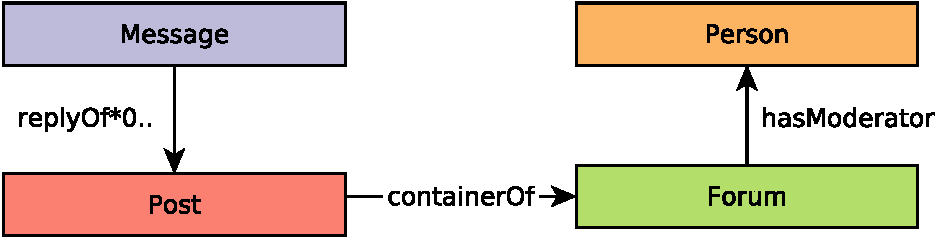
\includegraphics[scale=\patternscale,margin=0cm .2cm]{patterns/interactive-short-read-06}\hfill\vadjust{} \\ \hline
%
	desc. & Given a Message, retrieve the Forum that contains it and the Person that
moderates that forum. Since comments are not directly contained in
forums, for comments, return the forum containing the original post in
the thread which the comment is replying to.
 \\ \hline
%
	
%
    
        params &
        \innerCardVSpace{\begin{tabularx}{\attributeCardWidth}{|>{\paramNumberCell}c|>{\varNameCell}M|>{\typeCell}m{\typeWidth}|Y|} \hline
        \cellcolor{parameter} \color{white} \footnotesize $\mathsf{1}$ &Message.id& ID &  \\ \hline
        \end{tabularx}}\innerCardVSpace \\ \hline
	
%
	
        result &
        \innerCardVSpace{\begin{tabularx}{\attributeCardWidth}{|>{\resultNumberCell}c|>{\varNameCell}M|>{\typeCell}m{\typeWidth}|>{\resultOriginCell}c|Y|} \hline
        $\mathsf{1}$ & Message<-containerOf-Forum.id & ID &R&
                 \\ \hline
        $\mathsf{2}$ & Message<-containerOf-Forum.title & String &R&
                 \\ \hline
        $\mathsf{3}$ & Message<-containerOf-Forum-hasModerator->Person.id & ID &R&
                 \\ \hline
        $\mathsf{4}$ & Message<-containerOf-Forum-hasModerator->Person.firstName & String &R&
                 \\ \hline
        $\mathsf{5}$ & Message<-containerOf-Forum-hasModerator->Person.lastName & String &R&
                 \\ \hline
        \end{tabularx}}\innerCardVSpace \\ \hline
	
%
	%
	%
	%
    %
\end{tabularx}
\queryCardVSpace